\documentclass[tikz,border=6pt]{standalone}
\usepackage{tikz}
\usepackage{pgfplots}
\pgfplotsset{compat=1.18}
\pgfmathsetseed{20260422}
\begin{document}
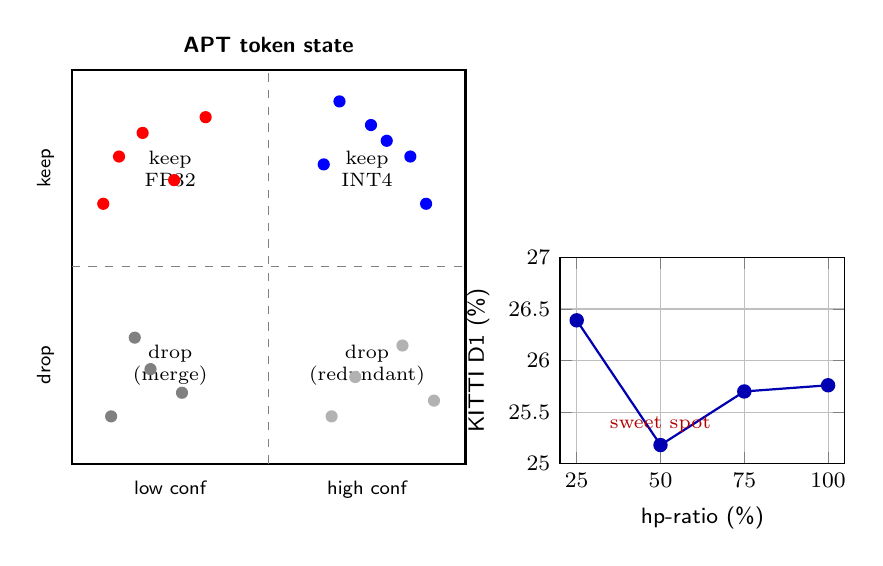
\begin{tikzpicture}[font=\sffamily\footnotesize]

% --- left: token-grid four-quadrant scatter ---
\begin{scope}
\draw[thick] (0,0) rectangle (5,5);
\draw[dashed,gray] (2.5,0) -- (2.5,5);
\draw[dashed,gray] (0,2.5) -- (5,2.5);
\node[below=1mm] at (1.25,0) {\scriptsize low conf};
\node[below=1mm] at (3.75,0) {\scriptsize high conf};
\node[left=1mm,rotate=90,anchor=south] at (0,1.25) {\scriptsize drop};
\node[left=1mm,rotate=90,anchor=south] at (0,3.75) {\scriptsize keep};
\node[above=1mm] at (2.5,5) {\textbf{APT token state}};

% quadrant labels
\node[align=center,font=\scriptsize] at (1.25,3.75) {keep\\FP32};
\node[align=center,font=\scriptsize] at (3.75,3.75) {keep\\INT4};
\node[align=center,font=\scriptsize] at (1.25,1.25) {drop\\(merge)};
\node[align=center,font=\scriptsize] at (3.75,1.25) {drop\\(redundant)};

% scatter dots (illustrative)
\foreach \x/\y/\c in {
  0.6/3.9/red,0.9/4.2/red,1.3/3.6/red,1.7/4.4/red,0.4/3.3/red,
  3.2/3.8/blue,3.8/4.3/blue,4.3/3.9/blue,3.4/4.6/blue,4.5/3.3/blue,4.0/4.1/blue,
  1.0/1.2/gray,0.8/1.6/gray,1.4/0.9/gray,0.5/0.6/gray,
  3.6/1.1/gray!60,4.2/1.5/gray!60,3.3/0.6/gray!60,4.6/0.8/gray!60}
  \fill[\c] (\x,\y) circle (2.2pt);
\end{scope}

% --- right: hp-ratio sweep inset ---
\begin{scope}[xshift=6.2cm]
\begin{axis}[
  width=5.2cm,height=4.2cm,
  font=\sffamily\footnotesize,
  xlabel={hp-ratio (\%)},
  ylabel={KITTI D1 (\%)},
  xmin=20,xmax=105,
  ymin=25,ymax=27,
  xtick={25,50,75,100},
  ytick={25,25.5,26,26.5,27},
  grid=major,
  mark options={scale=1.1},
  every axis plot/.append style={thick},
]
\addplot[color=blue!70!black,mark=*] coordinates {(25,26.39)(50,25.18)(75,25.70)(100,25.76)};
\node[above=1pt,font=\scriptsize,text=red!70!black] at (axis cs:50,25.18) {sweet spot};
\end{axis}
\end{scope}

\end{tikzpicture}
\end{document}
